\documentclass[12pt]{book}
\usepackage[utf8]{inputenc}
\usepackage[T1]{fontenc}
\usepackage{graphicx}
\usepackage{lipsum} % For dummy text
\usepackage{xcolor} % For colors
\usepackage{fancyhdr} % For header and footer customization
\usepackage{hyperref} % For hyperlinks in TOC and references
\usepackage{makeidx} % For index
\usepackage{tocloft} % For customizing TOC
\usepackage{amsmath} % For mathematical symbols if needed
\usepackage{appendix} % For appendix
\usepackage{biblatex} % For bibliography
\addbibresource{references.bib} % Bibliography file (replace references.bib with your .bib file)


%9910218400
%9899130865

% Set up header and footer
\pagestyle{fancy}
\fancyhf{}
\fancyhead[LE,RO]{\thepage}
\fancyhead[RE]{\leftmark}
\fancyhead[LO]{\rightmark}

% Customize chapter appearance
\usepackage{titlesec}
\definecolor{chaptercolor}{RGB}{51, 102, 153}
\titleformat{\chapter}[block]
  {\normalfont\Huge\bfseries\color{chaptercolor}}{\thechapter}{1em}{}

% Define color for links
\hypersetup{
    colorlinks=true,
    linkcolor=blue,
    filecolor=magenta,      
    urlcolor=cyan,
}

% For colorful Table of Contents
\renewcommand{\cftchapfont}{\color{chaptercolor}\bfseries}
\renewcommand{\cftchappagefont}{\color{chaptercolor}\bfseries}

% Index setup
\makeindex

% Begin document
\begin{document}

% Front Page
\begin{titlepage}
    \centering
    \vspace*{1in}
    {\Huge\bfseries\color{chaptercolor} Applied Statistics}\\
    \vspace{0.5in}
    {\Large\textit{R Sinuvasan}}\\
    \vfill
    
\includegraphics[width=0.5\textwidth]{VIT-AP LOGO} % Replace with actual image
    \vfill
    {\Large\textbf{Department of Mathematics}}\\
    \vspace{0.2in}
    {\Large 2024}
\end{titlepage}

% Title Page (Optional)
\newpage
\thispagestyle{empty}
\begin{center}
    \vspace*{1in}
    {\Huge\bfseries\color{chaptercolor} Applied Statistics}\\
    \vspace{0.5in}
    {\Large\textit{R Sinuvasan}}\\
    \vfill
    {\Large\textbf{Department of Mathematics}}\\
    \vspace{0.2in}
    {\Large 2024}
\end{center}
\newpage

% Preface
\chapter*{Preface}
\addcontentsline{toc}{chapter}{Preface}

In today’s data-driven world, the ability to analyze and interpret data is more critical than ever. Statistics provides the foundation for understanding data, while programming tools like R offer the computational power to perform complex analyses efficiently. This manual combines essential statistical concepts with hands-on R programming, offering students a comprehensive guide to both understanding and applying statistical techniques.

This manual is designed to introduce students to fundamental statistical methods and their implementation in R, enabling them to solve real-world problems using a practical, computational approach.

The first section focuses on descriptive statistics, covering measures of central tendency such as mean, median, and mode. These tools help summarize and interpret data, providing initial insights into datasets. R functions will be introduced to calculate these measures, allowing students to immediately see how statistical concepts translate into code.

We then explore probability theory, including key concepts like random events, conditional probability, and Bayes’ theorem. With R, students will simulate probabilistic scenarios and learn how to model uncertainty using code. Bayes’ theorem, in particular, will be implemented to demonstrate how new information updates probabilities in real time.

Next, the manual covers random variables and probability distributions, both discrete and continuous. In this section, students will learn how to work with common distributions (e.g., binomial, normal, Poisson) and use R to visualize and analyze these distributions. Simulations in R will help students gain a deeper understanding of how random variables behave and how distributions are used in practice.

Understanding relationships between variables is critical in data analysis, so we explore correlation and regression analysis. Using R, students will compute correlation coefficients and build regression models to investigate the strength and direction of relationships between variables. R’s graphical capabilities will also be employed to create scatter plots, residual plots, and other visualizations, making the results more interpretable.

In the final part of the manual, we focus on decision-making through hypothesis testing. Various tests, including the z-test, t-test, F-test, and chi-square test, will be covered. Each test will be demonstrated using R, guiding students through hypothesis formulation, execution of the tests, and interpretation of results. This hands-on approach ensures that students learn not only the theory but also the practical skills necessary for conducting statistical tests using real data.

Throughout this manual, R programming is integrated seamlessly with the statistical topics covered. By the end of the course, students will have a solid understanding of both statistical theory and how to use R to implement these techniques effectively. The focus on R not only equips students with a valuable skill for the job market but also enables them to work on data-driven projects with confidence.

Each chapter contains code snippets, exercises, and case studies to reinforce learning, ensuring that students can apply their knowledge to solve real-world problems. We hope this manual serves as a valuable resource, enabling students to harness the power of statistics and R programming in their academic and professional endeavors.

This version of the preface highlights how R programming is used throughout the manual to teach statistical concepts. It emphasizes the practical, hands-on approach that students will gain by combining theory with code, preparing them for real-world data analysis tasks.
\vspace{0.5in}
R Sinuvasan \\
October 2024

\newpage

% Table of Contents
\tableofcontents
\newpage

% Chapters
\chapter{Introduction}

In an age dominated by data, the ability to analyze and interpret information has become a critical skill across various fields, including business, healthcare, social sciences, and engineering. Statistics provides the essential framework for transforming raw data into meaningful insights, enabling informed decision-making. As we navigate through complex datasets, the integration of statistical theory with programming skills has proven invaluable. Among the tools available, \textbf{R} stands out as a powerful programming language specifically designed for statistical computing and data analysis.

R is an open-source programming language that has gained immense popularity among statisticians and data scientists for its robust capabilities and extensive ecosystem. It is renowned for its ability to handle complex statistical analyses, create compelling visualizations, and manage data effectively. With a vast array of packages available—such as \texttt{dplyr} for data manipulation, \texttt{ggplot2} for data visualization, and \texttt{tidyverse} for streamlined data science workflows—R empowers users to perform sophisticated statistical analyses with relative ease. Its flexibility and adaptability make it an essential tool for anyone working with data.

This manual is structured to provide a comprehensive overview of fundamental statistical concepts while employing R programming throughout. We will explore a variety of topics that are crucial for statistical analysis, including:

\begin{itemize}
    \item \textbf{Descriptive Statistics}: We begin by examining measures of central tendency—mean, median, and mode. These statistics summarize data sets, allowing us to draw initial insights about distributions. Through R, students will learn how to calculate and visualize these measures, gaining a deeper understanding of their significance.
    
    \item \textbf{Probability Theory}: Understanding probability is essential for making predictions based on data. This section introduces key concepts, including basic probability rules, conditional probability, and Bayes’ theorem. By using R to simulate probabilistic scenarios, students will learn to model uncertainty and apply Bayes’ theorem to real-world situations, enhancing their analytical skills.
    
    \item \textbf{Random Variables and Distributions}: We will delve into random variables and their associated probability distributions, exploring both discrete and continuous cases. This section will cover important distributions such as the binomial, normal, and Poisson distributions. R will be utilized to visualize these distributions and understand their applications in statistical analysis.
    
    \item \textbf{Correlation and Regression}: Understanding relationships between variables is crucial in data analysis. We will explore correlation coefficients and regression analysis, teaching students how to quantify relationships between variables. Using R, students will create regression models and visualizations, allowing them to make predictions based on their findings.
    
    \item \textbf{Hypothesis Testing and Decision Making}: The final section addresses hypothesis testing—a fundamental aspect of statistical analysis. Students will learn how to formulate and test hypotheses using z-tests, t-tests, F-tests, and chi-square tests. R will serve as a powerful tool for conducting these tests and interpreting the results, providing students with the skills to make informed decisions based on data.
\end{itemize}

By integrating R programming throughout the manual, we ensure that students not only grasp statistical theories but also develop practical coding skills essential for data analysis. Each chapter includes coding examples, exercises, and case studies that encourage students to apply their knowledge in real-world contexts.

The use of R in this manual is supported by a wealth of literature that showcases its capabilities and applications in statistics. For instance, \textit{R for Data Science} by Hadley Wickham and Garrett Grolemund provides an excellent introduction to data science concepts using R, guiding readers through practical data analysis techniques \cite{wickham2017r}. Furthermore, the R community continuously contributes to a growing repository of packages and resources, ensuring that users have access to the latest developments in statistical methodologies.

By the end of this manual, students will have a solid foundation in both statistical concepts and R programming, equipping them with the skills necessary to tackle diverse data-driven problems. We hope this resource inspires a deeper appreciation for the power of statistics and the role of R in unlocking insights from data.




\chapter{Introduction to R Programming}

\section{Introduction to R}

R is a programming language and environment primarily used for statistical computing and data analysis. It was developed by statisticians Ross Ihaka and Robert Gentleman at the University of Auckland, New Zealand, and has gained popularity among data analysts and researchers in various fields, including social sciences, bioinformatics, and finance.

R provides a wide range of statistical techniques and is highly extensible, allowing users to create custom functions and packages. As an open-source language, R has a large and active community that continuously contributes to its development and improvement. This community-driven approach has resulted in a vast ecosystem of packages available through the Comprehensive R Archive Network (CRAN), which enhances R's capabilities for various data analysis tasks.

The language is particularly known for its powerful data visualization tools, which enable users to create high-quality graphs and plots. R's syntax and data structures are designed to facilitate data manipulation, making it a preferred choice for exploratory data analysis.

R is also widely used for reproducible research, enabling analysts to produce dynamic reports that combine code, output, and narrative text, thus making the research process transparent and verifiable. 

Overall, R has become an essential tool for data scientists and statisticians, offering robust solutions for data analysis and visualization.

\begin{itemize}
    \item History and development of R.: R was developed in the early 1990s by statisticians Ross Ihaka and Robert Gentleman at the University of Auckland, New Zealand. It was designed as a free, open-source programming language for statistical computing and data analysis, inspired by the S programming language created by John Chambers and his colleagues at Bell Laboratories.

The first version of R was released in 1995, and it quickly gained traction within the statistical community. Its development was fueled by the growing need for powerful statistical tools that were accessible to researchers and analysts. In 2000, the R Project was formally established, and R became widely recognized as a leading language for statistical analysis and data visualization.

Over the years, R has evolved significantly, with contributions from a vibrant global community of developers and users. The Comprehensive R Archive Network (CRAN) was established as a repository for R packages, allowing users to share their work and access a vast array of additional functionalities.

Today, R is supported by a comprehensive ecosystem, including numerous packages for various statistical techniques, data manipulation, and visualization. Its adoption continues to grow in academia, industry, and government, making it one of the most popular tools for data analysis and research. 

    \item Advantages of using R for statistics and data analysis.: R offers several advantages for statisticians and data analysts:

\begin{itemize}
    \item \textbf{Open Source:} R is free to use and distribute, which makes it accessible to a wide range of users and encourages community contributions.
    \item \textbf{Comprehensive Statistical Packages:} R has a vast collection of packages available through CRAN, providing tools for a wide array of statistical analyses, from basic to advanced.
    \item \textbf{Data Visualization:} R excels in data visualization, with packages like \texttt{ggplot2} that allow users to create high-quality, customizable graphics.
    \item \textbf{Active Community:} A large and active community contributes to R’s development, providing support, resources, and continuously updated packages.
    \item \textbf{Reproducible Research:} R supports reproducible research through R Markdown, allowing users to combine code, analysis, and documentation in a single document.
    \item \textbf{Integration with Other Tools:} R can easily integrate with other programming languages (e.g., Python, C++), databases, and tools, enhancing its capabilities for data analysis.
    \item \textbf{User-Friendly Syntax:} The syntax of R is designed for data analysis, making it intuitive for statisticians and researchers, even those with limited programming experience.
\end{itemize}

    \item Overview of R’s ecosystem, including RStudio and CRAN.: R's ecosystem is rich and diverse, facilitating a wide range of statistical computing and data analysis tasks. Key components include:

\begin{itemize}
    \item \textbf{R:} The core programming language, designed for statistical analysis and data manipulation, with a wide array of built-in functions and libraries.
    \item \textbf{CRAN (Comprehensive R Archive Network):} A repository of R packages that extends R’s capabilities. It hosts thousands of packages for various statistical methods, data visualization, and machine learning.
    \item \textbf{RStudio:} An integrated development environment (IDE) that enhances the R programming experience. It offers features like syntax highlighting, debugging tools, and project management, making it easier for users to write and organize their R code.
    \item \textbf{R Markdown:} A tool for creating dynamic reports that combine R code with narrative text, enabling the presentation of data analysis results in an easily shareable format.
    \item \textbf{Bioconductor:} A project that provides tools for the analysis of genomic data, offering specialized packages for bioinformatics.
    \item \textbf{Shiny:} A web application framework for R that allows users to create interactive web applications directly from R, making data analysis accessible to non-programmers.
\end{itemize}

This ecosystem collectively empowers users to perform complex data analyses, create reproducible research, and visualize results effectively.


\end{itemize}

\section{Installing R and RStudio}
To get started with R, you first need to install R and RStudio.
\begin{itemize}
    \item Step-by-step instructions for installing R and RStudio.
    \item Overview of R packages and how to install them using \texttt{install.packages()}.
    \item Basic configuration tips for RStudio.
\end{itemize}

\section{Installing R}
\subsection{Windows}
To install R on Windows:
\begin{itemize}
    \item Visit the \href{https://cran.r-project.org/bin/windows/base/}{CRAN Windows page}.
    \item Click on the download link for the latest version of R.
    \item Run the installer and follow the on-screen instructions, leaving most options at their default values unless you have specific needs.
\end{itemize}

\subsection{Mac OS X}
For Mac users:
\begin{itemize}
    \item Go to the \href{https://cran.r-project.org/bin/macosx/}{CRAN Mac OS page}.
    \item Download the most recent version of the \texttt{.pkg} file (e.g., \texttt{R-4.3.0.pkg}).
    \item Open the file and follow the installer instructions to complete the installation.
\end{itemize}

\subsection{Linux}
On Linux-based systems, R can be installed using the terminal:
\begin{itemize}
    \item Open a terminal window.
    \item For Debian-based distributions (e.g., Ubuntu), use the command:
    \begin{verbatim}
    sudo apt-get install r-base
    \end{verbatim}
    \item For Fedora-based distributions, use:
    \begin{verbatim}
    sudo dnf install R
    \end{verbatim}
    \item Ensure that any dependencies required by R are installed.
\end{itemize}

\section{Installing RStudio}
Once R is installed, you can install RStudio:
\begin{itemize}
    \item Visit the \href{https://www.rstudio.com/products/rstudio/download/#download}{RStudio download page}.
    \item Choose your operating system (Windows, Mac, or Linux) and download the corresponding installer.
    \item Run the installer and follow the on-screen instructions to set up RStudio.
\end{itemize}

\subsection{Windows and Mac}
For both Windows and Mac, the installation is straightforward: download the executable file, open it, and proceed with the default options unless specific configurations are needed.

\subsection{Linux}
On Linux, after downloading the \texttt{.deb} or \texttt{.rpm} file, use the terminal to install RStudio:
\begin{itemize}
    \item For Debian-based systems, run:
    \begin{verbatim}
    sudo dpkg -i rstudio-x.yy.zzz-amd64.deb
    \end{verbatim}
    \item For Fedora-based systems, run:
    \begin{verbatim}
    sudo dnf install rstudio-x.yy.zzz-x86_64.rpm
    \end{verbatim}
    \item Replace \texttt{x.yy.zzz} with the actual version number of RStudio you downloaded.
\end{itemize}

\section{Overview of R Packages}
R packages are collections of R functions, data, and compiled code that are stored in a well-defined format. They extend R's functionality by providing tools for specific tasks, such as data manipulation, visualization, or statistical analysis. Many packages are available through CRAN (Comprehensive R Archive Network), but others are hosted on platforms like GitHub.

\section{Installing R Packages}
To install an R package, use the \texttt{install.packages()} function. This function downloads and installs the specified package from CRAN or other repositories.

\subsection{Example of Installing a Package}
For example, to install the \texttt{ggplot2} package for data visualization, run the following command in your R console:
\begin{verbatim}
install.packages("ggplot2")
\end{verbatim}
This command will download and install the package, including any dependencies, automatically.

\subsection{Loading an Installed Package}
Once a package is installed, load it into your R session using the \texttt{library()} function:
\begin{verbatim}
library(ggplot2)
\end{verbatim}

\section{Commonly Used Packages}
Some widely-used packages in R include:
\begin{itemize}
    \item \texttt{dplyr} – for data manipulation
    \item \texttt{ggplot2} – for data visualization
    \item \texttt{tidyverse} – a collection of data science tools
    \item \texttt{shiny} – for building interactive web applications
\end{itemize}




\section{Basic Configuration Tips for RStudio}
\begin{itemize}
    \item \textbf{Appearance:} Go to \texttt{Tools > Global Options > Appearance} to change the editor theme and font size for better visibility.
    \item \textbf{Pane Layout:} Customize the layout of RStudio panes (Source, Console, Environment) under \texttt{Tools > Global Options > Pane Layout}.
\end{itemize}

\section{Code Execution}
\begin{itemize}
    \item Enable line numbers, auto-complete, and code folding under \texttt{Tools > Global Options > Code}.
    \item Set keyboard shortcuts for running code chunks (e.g., \texttt{Ctrl + Enter}).
\end{itemize}

\section{Packages}
\begin{itemize}
    \item Manage installed packages via the \texttt{Packages} tab or use \texttt{install.packages()} to add new packages.
\end{itemize}





\section{Basic R Syntax}
Understanding the basic syntax of R is crucial for efficient programming.
\begin{itemize}
    \item Variables, data types (numeric, character, factor, logical).
    \item Basic operators (arithmetic, relational, logical).
    \item Introduction to vectors and data frames.
\end{itemize}





\section{Variables in R}
Variables in R are used to store data that can be manipulated during the execution of a program. A variable can be assigned a value using the assignment operator \texttt{<-} or \texttt{=}. For example:
\begin{verbatim}
x <- 10
name <- "John"
\end{verbatim}
In R, variables do not need explicit declaration, and their type is determined dynamically when a value is assigned.

\section{Data Types in R}
R provides several basic data types that are essential for handling different kinds of data. These include numeric, character, factor, and logical types.

\subsection{Numeric}
The numeric data type is used to store numbers, both integers and real numbers (decimals). For example:
\begin{verbatim}
x <- 42
y <- 3.14
\end{verbatim}
R treats all numbers as double precision by default, but integers can also be explicitly declared using the \texttt{as.integer()} function.

\subsection{Character}
Character data represents text or strings. Characters are enclosed in double or single quotes. For example:
\begin{verbatim}
name <- "Alice"
greeting <- 'Hello'
\end{verbatim}

\subsection{Factor}
Factors are used to handle categorical data in R. They store both the values and the possible categories. Factors are particularly useful for statistical modeling:
\begin{verbatim}
colors <- factor(c("red", "blue", "green", "red"))
\end{verbatim}
Factors can be ordered or unordered and are often used in data frames for analysis.

\subsection{Logical}
Logical data types store boolean values: \texttt{TRUE} or \texttt{FALSE}. They are often the result of comparisons or logical operations:
\begin{verbatim}
is_sunny <- TRUE
result <- 5 > 3  # result will be TRUE
\end{verbatim}


Understanding variables and data types is crucial for working effectively with R. The dynamic nature of R allows for flexible handling of different types of data, making it easier to perform statistical analysis and data manipulation.







\section{Introduction}
In R, operators allow you to perform various computations on data. These include arithmetic operations for numerical calculations, relational operators for comparisons, and logical operators for evaluating boolean expressions. Understanding these operators is fundamental for programming in R.

\section{Arithmetic Operators}
Arithmetic operators are used for basic mathematical computations. The main arithmetic operators in R are:
\begin{itemize}
    \item \texttt{+} : Addition
    \item \texttt{-} : Subtraction
    \item \texttt{*} : Multiplication
    \item \texttt{/} : Division
    \item \texttt{\^} : Exponentiation
    \item \texttt{\%/\%} : Integer division (quotient)
    \item \texttt{\%\%} : Modulo (remainder)
\end{itemize}



\subsection{Examples}
\begin{verbatim}
x <- 10
y <- 3

sum <- x + y        # sum = 13
diff <- x - y       # diff = 7
prod <- x * y       # prod = 30
quot <- x / y       # quot = 3.33
exp <- x ^ y        # exp = 1000
int_div <- x %/% y  # int_div = 3
mod <- x %% y       # mod = 1
\end{verbatim}

\section{Relational Operators}
Relational operators compare values and return \texttt{TRUE} or \texttt{FALSE}. The main relational operators are:
\begin{itemize}
    \item \texttt{==} : Equal to
    \item \texttt{!=} : Not equal to
    \item \texttt{>} : Greater than
    \item \texttt{<} : Less than
    \item \texttt{>=} : Greater than or equal to
    \item \texttt{<=} : Less than or equal to
\end{itemize}

\subsection{Examples}
\begin{verbatim}
x <- 5
y <- 10

result1 <- x == y    # result1 = FALSE
result2 <- x != y    # result2 = TRUE
result3 <- x > y     # result3 = FALSE
result4 <- x <= y    # result4 = TRUE
\end{verbatim}

Relational operators are often used in conditions for \texttt{if} statements, loops, and other control structures.

\section{Logical Operators}
Logical operators evaluate logical expressions and are primarily used to combine relational operations. The main logical operators are:
\begin{itemize}
    \item \texttt{\&} : Logical AND
    \item \texttt{|} : Logical OR
    \item \texttt{!} : Logical NOT
\end{itemize}

\subsection{Examples}
\begin{verbatim}
a <- TRUE
b <- FALSE

result1 <- a & b     # result1 = FALSE (both must be TRUE)
result2 <- a | b     # result2 = TRUE (one must be TRUE)
result3 <- !a        # result3 = FALSE (logical negation)
\end{verbatim}

Logical operators are especially useful when you need to check multiple conditions.


Arithmetic, relational, and logical operators are crucial in R for data manipulation, decision-making, and computations. They provide a foundation for writing effective R scripts and performing complex analyses.




\section{Vectors in R}
A vector is one of the most basic data structures in R. It is a sequence of data elements of the same type, such as numeric, character, or logical. Vectors can be created using the \texttt{c()} function, which combines values into a single vector.

\subsection{Example of a Numeric Vector}
\begin{verbatim}
numbers <- c(1, 2, 3, 4, 5)
\end{verbatim}
Vectors in R are 1-dimensional and are fundamental to most data manipulation operations.

\subsection{Example of a Character Vector}
\begin{verbatim}
names <- c("Alice", "Bob", "Charlie")
\end{verbatim}



In this chapter, we will cover vectors. A vector is a data structure in R. A data structure can be defined as a collection of data values, the relationships among them, and the functions or operations that can be applied to the data. A vector can either be an atomic vector or a list. An atomic vector contains only one data type, whereas a list may contain multiple data types.

An atomic vector could be Character, Logical, Double, Integer, or Complex.

\subsection{Integer}
\begin{verbatim}
4
## [1] 4
\end{verbatim}

\subsection{Character}
\begin{verbatim}
"Pune"
## [1] "Pune"
\end{verbatim}

You can use the \texttt{typeof} function to check the type of each of these:
\begin{verbatim}
typeof("Pune")
## [1] "character"
typeof(4)
## [1] "double"
typeof(4.3)
## [1] "double"
typeof(2+1i) 
## [1] "complex"
\end{verbatim}

\subsection{Creating a Vector}
Let's create a vector containing three numeric values. This will be an example of a Numeric Vector:
\begin{verbatim}
c(1, 4, 7)
## [1] 1 4 7
\end{verbatim}

To check the length of the vector, we can use the length function:
\begin{verbatim}
length(c(1, 4, 7))
## [1] 3
\end{verbatim}

Let's assign this to a variable for future use:
\begin{verbatim}
Num_variable <- c(1, 4, 7)
\end{verbatim}

Let’s create a vector \texttt{Names} that contains the names of persons appearing in an Exam. This will be a kind of character vector. Please note that here \texttt{Names} is a vector, and \texttt{<-} is an operator that assigns the value on the right-hand side of the operator to the variable name on the left-hand side. The character \texttt{c} is used to create a vector:
\begin{verbatim}
Names <- c("Arvind", "Krishna", "Rahul", "Saurabh", "Venkat", "Sucharitha")
\end{verbatim}

Let's extract the first element of the \texttt{Names} vector. To extract the first element, we need to use \texttt{[} and the value 1:
\begin{verbatim}
Names[1]
## [1] "Arvind"
\end{verbatim}

Similarly, to extract the third value from the \texttt{Names} vector:
\begin{verbatim}
Names[3]
## [1] "Rahul"
\end{verbatim}

Let’s create another vector and see if we can combine two vectors:
\begin{verbatim}
Missed_names <- c("Ajay", "Amit")
\end{verbatim}

Here we will be updating the \texttt{Names} vector by including \texttt{Missed\_names} in the \texttt{Names} vector:
\begin{verbatim}
Names <- c(Names, Missed_names)
Names
## [1] "Arvind"     "Krishna"    "Rahul"      "Saurabh"    "Venkat"    
## [6] "Sucharitha" "Ajay"       "Amit"
\end{verbatim}

\subsection{Class of Vector}
We can also check the types of vectors using different functions such as:
\begin{verbatim}
class(Names)
## [1] "character"
class(Num_variable)
## [1] "numeric"
typeof(Num_variable)
## [1] "double"
\end{verbatim}

What is the difference between \texttt{typeof}, \texttt{mode}, and \texttt{class}? I will leave it to the reader to explore it on their own. Remember the reader can use the \texttt{help} function to check the definitions in detail. For example, just type \texttt{?class} in the console to see the details of the class function.

\subsection{Adding Vectors of Different Types}
Let’s add a character and numeric vector and check the result:
\begin{verbatim}
mix_vector <- c(1, 2, "Amish")
class(mix_vector)
## [1] "character"
\end{verbatim}

The \texttt{mix\_vector} we created had multiple data types (Numeric and Character); however, R converts the multiple data types to a single data type through a process called coercion. Logical values are converted to numbers: TRUE is converted to 1 and FALSE to 0.

Values are converted to the simplest type required to represent all information.

The ordering is roughly logical < integer < numeric < complex < character < list.

Objects of type \texttt{raw} are not converted to other types.

Objects can also be explicitly coerced using the \texttt{as.} function. For example, to coerce the \texttt{mix\_vector} to numeric use:
\begin{verbatim}
mix_vector <- as.numeric(mix_vector)
## Warning: NAs introduced by coercion
mix_vector
## [1]  1  2 NA
class(mix_vector)
## [1] "numeric"
\end{verbatim}

We can also change the elements of the vector. Let’s change the first element of the \texttt{Names} vector using the following expression:
\begin{verbatim}
Names[1] <- "Arun"
Names
## [1] "Arun"       "Krishna"    "Rahul"      "Saurabh"    "Venkat"    
## [6] "Sucharitha" "Ajay"       "Amit"
\end{verbatim}

\subsection{Accessing Elements of Vectors}
Let’s try to access elements of the vector using negative indexing:
\begin{verbatim}
Names[-1] # All elements except the first element will be printed
## [1] "Krishna"    "Rahul"      "Saurabh"    "Venkat"     "Sucharitha"
## [6] "Ajay"       "Amit"
Names[c(-1, -2)] # All elements except the first and second elements will be printed
## [1] "Rahul"      "Saurabh"    "Venkat"     "Sucharitha" "Ajay"      
## [6] "Amit"
\end{verbatim}

Alternatively, we can also use the following code to remove the first two elements of the \texttt{Names} vector:
\begin{verbatim}
Names[-c(1, 2)] # All elements except the first and second elements will be printed
## [1] "Rahul"      "Saurabh"    "Venkat"     "Sucharitha" "Ajay"      
## [6] "Amit"
\end{verbatim}

\subsection{Creating Vector Using In-Built Functions}
\begin{verbatim}
seq(1, 10, by = 1) # Create a sequential vector from 1 to 10 which increases by 1 in length.
##  [1]  1  2  3  4  5  6  7  8  9 10
seq(1, 10, by = 0.5)
##  [1]  1.0  1.5  2.0  2.5  3.0  3.5  4.0  4.5  5.0  5.5  6.0  6.5  7.0  7.5
## [15]  8.0  8.5  9.0  9.5 10.0
\end{verbatim}

\subsection{Let’s Try to Repeat Vectors}
\begin{verbatim}
rep(c(1, 2), times = c(5, 5))
##  [1] 1 1 1 1 1 2 2 2 2 2
\end{verbatim}

\texttt{typeof(Vector)}: This method tells you the data type of the vector.

\texttt{Sort(Vector)}: This method helps us to sort the items in ascending order.

\texttt{length(Vector)}: This method counts the number of elements in a vector.

\texttt{head(Vector, limit)}: This method returns the top six elements (if you omit the limit). If you specify the limit as 4, then it returns the first 4 elements.

\texttt{tail(Vector, limit)}: It returns the last six elements (if you omit the limit). If you specify the limit as 2, then it returns the last two elements.

\subsection{Arithmetic Operators in Vectors in R}

We have performed arithmetic operations in previous chapters. Let’s see how we can perform arithmetic operations in vectors.

\begin{verbatim}
V1 <- c(1, 2, 3, 4) # created a vector V1 
V2 <- c(5, 6, 7, 8) # created a vector V2
\end{verbatim}

Let's perform addition:
\begin{verbatim}
V12 <- V1 + V2
V12 # Print result of V12, which is sum of V1 and V2 vector.
## [1]  6  8 10 12
\end{verbatim}

As you may have guessed, the addition operation above was performed elementwise. That means that the first element of \texttt{V1} was added to the first element of \texttt{V2}.

Let’s perform multiplication:
\begin{verbatim}
V12_mult <- V1 * V2
V12_mult
## [1]  5 12 21 32
\end{verbatim}

Let’s perform division:
\begin{verbatim}
V12_division <- V2 / V1
V12_division
## [1] 5.000000 3.000000 2.333333 2.000000
typeof(V12_division)
## [1] "double"
\end{verbatim}

Let’s convert the double to numeric:
\begin{verbatim}
V12_division <- as.integer(V12_division)
V12_division
## [1] 5 3 2 2
typeof(V12_division)
## [1] "integer"
\end{verbatim}







%\section{Data Frames in R}
%A data frame is a table or a 2-dimensional array-like structure in which each column contains values of one variable, and each row represents an observation. Each column can have different data types, making data frames essential for handling datasets in R.
%
%\subsection{Creating a Data Frame}
%\begin{verbatim}
%df <- data.frame(Name = c("Alice", "Bob"), Age = c(25, 30))
%\end{verbatim}
%Data frames are widely used for data analysis, especially when handling structured datasets such as those found in spreadsheets.
%
%
%Vectors and data frames are foundational data structures in R. Vectors store sequences of the same data type, while data frames are ideal for storing datasets with different types across columns.
%
%
%
%
%
%
%\section{Data Frames}
%Understanding data frames as a primary data structure in R.
%\begin{itemize}
%    \item Creating data frames and manipulating them using \texttt{data.frame()} and related functions.
%    \item Accessing and subsetting data frames.
%\end{itemize}
%
%\section{Matrices}
%Introduction to matrices as a data structure in R.
%\begin{itemize}
%    \item Creating matrices using \texttt{matrix()}, and performing operations.
%    \item Differences between matrices and data frames.
%\end{itemize}



\section{Introduction to Data Frames in R}

Data frames in R language are a type of data structure used to store data in a tabular form, which is two-dimensional. The data frames are a special category of list data structures in which the components are of equal length. R language supports the built-in function \texttt{data.frame()} to create data frames and assign data elements. R also supports using the data frame name to modify and retrieve data elements from data frames. Data frames in R are structured with column names as component names, and rows structured by component values. Data frames in R are a widely used data structure when developing machine learning models in data science projects.

\subsection{Characteristics of Data Frames}
\begin{itemize}
    \item The column name is required.
    \item Row names should be unique.
    \item The number of items in each column should be the same.
\end{itemize}

\section{Steps For Creating Data Frames in R}

Let’s start with creating a data frame, which is explained below:

\subsection{Step 1: Create a Data Frame of a Class in a School}
\textbf{Code:}
\begin{verbatim}
tenthclass = data.frame(roll_number = c(1:5),
Name = c("John","Sam","Casey","Ronald","Mathew"),
Marks = c(77,87,45,68,95), stringsAsFactors = FALSE)
print(tenthclass)
\end{verbatim}

When we run this code, we will get a data frame like this:

\textbf{Output:}

\begin{figure}[h]
    \begin{flushleft}
        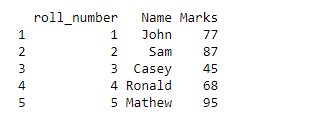
\includegraphics[width=0.7\textwidth]{Data-Frames-in-R-1-1.png} % Image file
        \caption{Data frame output example}
        \label{fig:dataframe}
    \end{flushleft}
\end{figure}
Here, in our example, the data frame is very small, but in real life, while dealing with problems, we have lots of data. To understand the structure of the data, we use the \texttt{Str()} function.

\subsection{Step 2: Add the following line to our code}

\textbf{Code:}
\begin{verbatim}
Str(tenthclass)
\end{verbatim}

When we run the whole code, we will get the following output:

\textbf{Output:}
\begin{figure}[h]
    \begin{flushleft}
        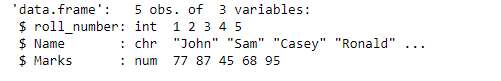
\includegraphics[width=0.7\textwidth]{Data-Frames-in-R-1-2.png} % Image file
        \caption{Data frame output example}
        \label{fig:dataframe}
    \end{flushleft}
\end{figure}

The above output means we have 5 observations of 3 variables. It also explains the data type of each variable. For example, the roll number is an integer, the name is a character, and Marks are numeric.

Once we understand the structure of the data, we can pass the following code to understand the data more statistically.

\subsection{Step 3: Use the \texttt{summary()} Function}

\textbf{Code:}
\begin{verbatim}
summary(tenthclass)
\end{verbatim}

\textbf{Output:}
\begin{figure}[h]
    \begin{flushleft}
        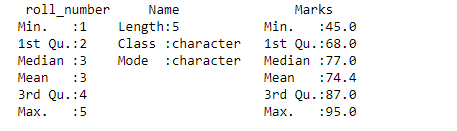
\includegraphics[width=0.7\textwidth]{Data-Frames-in-R-1-3.png} % Image file
        \caption{Data frame output example}
        \label{fig:dataframe}
    \end{flushleft}
\end{figure}

The \texttt{summary()} function provides a better understanding of our data. It tells us the mean, median, quartiles, maximum, and minimum values, helping us make better decisions.













\section{Matrices in R}

Matrices are two-dimensional data structures in R and are arranged in a rectangular layout. Matrices can contain only one data type. We can create matrices of any of the six data types we discussed before. A matrix can also be thought of as a vector in two dimensions.

We can use the \texttt{matrix} function to create a matrix in R programming. I will suggest using \texttt{? matrix} for detailed documentation of the matrix function. Let’s create a matrix with 3 rows and 2 columns:

\begin{verbatim}
matrix(1:6, nrow = 3, ncol = 2)
##      [,1] [,2]
## [1,]    1    4
## [2,]    2    5
## [3,]    3    6
\end{verbatim}

What if we don’t specify the number of rows and columns?

\begin{verbatim}
matrix(1:6, 3, 2)
##      [,1] [,2]
## [1,]    1    4
## [2,]    2    5
## [3,]    3    6
\end{verbatim}

As you have guessed from the above output, R will automatically pick the number of rows and columns based on the order of input. Let’s specify one of the dimensions (either column or row) and see the output:

\begin{verbatim}
matrix(1:6, ncol = 3)
##      [,1] [,2] [,3]
## [1,]    1    3    5
## [2,]    2    4    6
\end{verbatim}

So far we have not assigned any column names and row names to the matrix. Let’s create a matrix \( M \) and assign column names and row names:

\begin{verbatim}
M <- matrix(1:20, ncol = 4)
colnames(M) <- c("A", "B", "C", "D")
rownames(M) <- c("E", "F", "G", "H", "I")
\end{verbatim}

Let’s check the matrix \( M \):

\begin{verbatim}
M
##   A  B  C  D
## E 1  6 11 16
## F 2  7 12 17
## G 3  8 13 18
## H 4  9 14 19
## I 5 10 15 20
\end{verbatim}

As you can see from the output, we have successfully assigned names to the columns. We can also call specific columns now. For example, \texttt{Matrix[rowname, colname]} will call the required row and column by name:

\begin{verbatim}
M["F", "D"]
## [1] 17
\end{verbatim}

We can leave the row name field blank in \texttt{Matrix[rowname, colname]} to call the complete column:

\begin{verbatim}
M[, "D"]
##  E  F  G  H  I 
## 16 17 18 19 20
\end{verbatim}

As you can see in the above example, we have kept the row blank. This will cause the above expression to pick all the values from the corresponding columns. We can also access specific elements of vectors by specifying the row number and column number. Let’s say we want to pick a specific column and vector from matrix, say the 2nd row and 3rd column:

\begin{verbatim}
M[2, 3]
## [1] 12
\end{verbatim}

\subsection{Extracting Row/Column from Matrices}

We can also extract more than one row or column at a time. For example, below we extracted the first and third column and the second row:

\begin{verbatim}
M[2, c(1, 3)]
##  A  C 
##  2 12
\end{verbatim}

So what else can we do with matrices?

\subsection{Operations in Matrices}

Let’s perform some operations with matrices. Let’s create two matrices \( M_1 \) and \( M_2 \) and perform some operations:

\begin{verbatim}
M1 <- matrix(1:15, nrow = 5)
M1
##      [,1] [,2] [,3]
## [1,]    1    6   11
## [2,]    2    7   12
## [3,]    3    8   13
## [4,]    4    9   14
## [5,]    5   10   15

M2 <- matrix(1:15, nrow = 5)
M2
##      [,1] [,2] [,3]
## [1,]    1    6   11
## [2,]    2    7   12
## [3,]    3    8   13
## [4,]    4    9   14
## [5,]    5   10   15
\end{verbatim}

\subsubsection{Arithmetic Operations in Matrices}

What if we add two matrices? Matrix operations can be performed similarly to how arithmetic operations are performed on numbers. However, we should be careful with the dimensions of the matrices that we are working on.

Let’s create three matrices \( M_1, M_2, M_3 \):

\begin{verbatim}
M1 <- matrix(1:15, nrow = 5)
M1
##      [,1] [,2] [,3]
## [1,]    1    6   11
## [2,]    2    7   12
## [3,]    3    8   13
## [4,]    4    9   14
## [5,]    5   10   15

M2 <- matrix(2:16, nrow = 5)
M2
##      [,1] [,2] [,3]
## [1,]    2    7   12
## [2,]    3    8   13
## [3,]    4    9   14
## [4,]    5   10   15
## [5,]    6   11   16

M3 <- matrix(2:10, nrow = 5)
## Warning in matrix(2:10, nrow = 5): data length [9] is not a sub-multiple or
## multiple of the number of rows [5]
M3
##      [,1] [,2]
## [1,]    2    7
## [2,]    3    8
## [3,]    4    9
## [4,]    5   10
## [5,]    6    2
\end{verbatim}

\textbf{Arithmetic Operations in Matrices}

Addition operation on matrices of the same dimension:

\begin{verbatim}
M1 + M2
##      [,1] [,2] [,3]
## [1,]    3   13   23
## [2,]    5   15   25
## [3,]    7   17   27
## [4,]    9   19   29
## [5,]   11   21   31
\end{verbatim}

What if we want to add matrices of different dimensions? We can check the dimensions of matrices using the \texttt{dim} function:

\begin{verbatim}
dim(M1)
## [1] 5 3
dim(M3)
## [1] 5 2
\end{verbatim}

Multiplying matrices of the same dimension: The following operation using \texttt{"*"} is element-wise:

\begin{verbatim}
M1 * M2
##      [,1] [,2] [,3]
## [1,]    2   42  132
## [2,]    6   56  156
## [3,]   12   72  182
## [4,]   20   90  210
## [5,]   30  110  240
\end{verbatim}
What if we want Matrix Multiplication? As an exercise, try \texttt{M1\%*\%M2} in the R console for matrix multiplication and check the result. Once you run the operation, you must have got an error message ``Error in M1 \%*\% M2: non-conformable arguments". Why is it so? As a basic rule for matrix multiplication, the number of rows of Matrix1 should be equal to the number of columns in Matrix2 when multiplying Matrix1 with Matrix2. You can check the following link \textit{mathisfun}.

\begin{verbatim}
M4 <- matrix(1:9, nrow=3)
M5 <- matrix(10:18, nrow=3)
M4
\end{verbatim}
\begin{verbatim}
##      [,1] [,2] [,3]
## [1,]    1    4    7
## [2,]    2    5    8
## [3,]    3    6    9
\end{verbatim}
\begin{verbatim}
M5
\end{verbatim}
\begin{verbatim}
##      [,1] [,2] [,3]
## [1,]   10   13   16
## [2,]   11   14   17
## [3,]   12   15   18
\end{verbatim}
Let's see the result of Matrix Multiplication:

\begin{verbatim}
M4 <- matrix(1:9, nrow=3)
M5 <- matrix(10:18, nrow=3)
M4 \%*\% M5
\end{verbatim}
\begin{verbatim}
##      [,1] [,2] [,3]
## [1,]  138  174  210
## [2,]  171  216  261
## [3,]  204  258  312
\end{verbatim}
You can see the elementwise operation result in R:

\begin{verbatim}
M4 * M5
\end{verbatim}
\begin{verbatim}
##      [,1] [,2] [,3]
## [1,]   10   52  112
## [2,]   22   70  136
## [3,]   36   90  162
\end{verbatim}
\begin{verbatim}
M1 / M2
\end{verbatim}
\begin{verbatim}
##           [,1]      [,2]      [,3]
## [1,] 0.5000000 0.8571429 0.9166667
## [2,] 0.6666667 0.8750000 0.9230769
## [3,] 0.7500000 0.8888889 0.9285714
## [4,] 0.8000000 0.9000000 0.9333333
## [5,] 0.8333333 0.9090909 0.9375000
\end{verbatim}
What if one of the matrices' row or column is shorter than the other? Will recycling occur?

As an exercise, create a 3X3 matrix and add it to M1.

\subsection{Transposing a Matrix}
You may also want to transpose your data in R. This is used to interchange rows and columns, i.e., rows become columns and columns become rows in the new transposed matrix. For example:

\begin{verbatim}
M3 <- t(M1)
M3
\end{verbatim}
\begin{verbatim}
##      [,1] [,2] [,3] [,4] [,5]
## [1,]    1    2    3    4    5
## [2,]    6    7    8    9   10
## [3,]   11   12   13   14   15
\end{verbatim}
As you can see from the output, the rows have become columns and the columns have become rows. This can also be used to reshape a DataFrame. We will cover DataFrame in the next chapter.

\subsection{Common Matrix Operations in R}
Sum of rows in Matrix:
\begin{verbatim}
rowSums(M1)
\end{verbatim}
\begin{verbatim}
## [1] 18 21 24 27 30
\end{verbatim}

Sum of columns in Matrix:
\begin{verbatim}
colSums(M1)
\end{verbatim}
\begin{verbatim}
## [1] 15 40 65
\end{verbatim}

Mean of rows in Matrix:
\begin{verbatim}
rowMeans(M1)
\end{verbatim}
\begin{verbatim}
## [1]  6  7  8  9 10
\end{verbatim}

\subsection{Naming Matrix Rows and Columns}
\begin{verbatim}
rownames(M4) <- c("A","B","C")
colnames(M4) <- c("D","E","F")
M4
\end{verbatim}
\begin{verbatim}
##   D E F
## A 1 4 7
## B 2 5 8
## C 3 6 9
\end{verbatim}

We can also extract specific elements of a Matrix by specifying rows and columns:

\begin{verbatim}
M4[3,] % # Extracting third row from Matrix M4
\end{verbatim}
\begin{verbatim}
## D E F 
## 3 6 9
\end{verbatim}
\begin{verbatim}
M4[,3] % # Extracting third column from Matrix M4
\end{verbatim}
\begin{verbatim}
## A B C 
## 7 8 9
\end{verbatim}
\begin{verbatim}
M4[2,3] % # Extracting second row and third column element from Matrix M4
\end{verbatim}
\begin{verbatim}
## [1] 8
\end{verbatim}










\section{Functions in R}
Introduction to functions: syntax and structure.
\begin{itemize}
    \item Writing custom functions in R.
    \item Understanding scope and return values.
    \item Using built-in functions and applying functions like \texttt{apply()}, \texttt{lapply()}, etc.
\end{itemize}

\section{Data Import and Export}
R provides various functions for importing and exporting data.
\begin{itemize}
    \item Reading data into R from various sources (CSV, Excel, databases).
    \item Writing data to files (CSV, Excel).
    \item Using packages like \texttt{readr}, \texttt{openxlsx}, and \texttt{DBI}.
\end{itemize}

\section{Data Manipulation}
Using the \texttt{dplyr} package allows for streamlined data manipulation.
\begin{itemize}
    \item Key functions: \texttt{filter()}, \texttt{select()}, \texttt{mutate()}, \texttt{arrange()}, \texttt{summarize()}.
    \item Piping (\texttt{\%>\%}) and its advantages in data processing.
\end{itemize}

\section{Data Visualization}
Data visualization is vital for interpreting statistical results.
\begin{itemize}
    \item Introduction to the \texttt{ggplot2} package.
    \item Creating various plots: scatter plots, histograms, boxplots, etc.
    \item Customizing plots (labels, colors, themes).
\end{itemize}

\section{Programming with R}
In addition to statistical functions, R allows for traditional programming constructs.
\begin{itemize}
    \item Control structures: loops (\texttt{for}, \texttt{while}), conditionals (\texttt{if}, \texttt{else}).
    \item Writing functions and understanding scope.
    \item Error handling and debugging techniques.
\end{itemize}

\section{Working with Packages}
Packages enhance R's capabilities, providing additional functions.
\begin{itemize}
    \item How to find and use R packages.
    \item Overview of essential packages for statistics (e.g., \texttt{MASS}, \texttt{caret}, \texttt{tidyverse}).
    \item How to check package documentation and help files.
\end{itemize}

\section{R Markdown}
R Markdown is a powerful tool for creating dynamic reports.
\begin{itemize}
    \item Creating dynamic reports that combine code and output.
    \item Exporting reports to different formats (HTML, PDF, Word).
\end{itemize}

\section{Basic Project Structure}
Organizing R projects for better workflow is essential.
\begin{itemize}
    \item Using RStudio projects for file management and version control.
    \item Best practices for coding in R.
\end{itemize}

\section{Resources for Learning R}
Numerous resources are available for those who wish to deepen their knowledge.
\begin{itemize}
    \item Recommended books, online courses, and tutorials for further learning.
    \item Community resources and forums (e.g., R-bloggers, Stack Overflow).
\end{itemize}

\section{Advanced Topics (Optional)}
For advanced users, R offers powerful features for machine learning and large datasets.
\begin{itemize}
    \item Introduction to advanced statistical methods in R (e.g., machine learning with \texttt{caret} or \texttt{mlr}).
    \item Working with large datasets using \texttt{data.table}.
    \item Building shiny applications for interactive data visualization.
\end{itemize}



% Appendix
\appendix
\chapter{Appendix A: LaTeX Resources}
Here are some useful resources to help you further explore LaTeX:

\begin{itemize}
    \item \href{https://www.latex-project.org/}{LaTeX Project Official Website}
    \item \href{https://www.overleaf.com/learn}{Overleaf LaTeX Documentation}
\end{itemize}

\index{Resources} % Adding to the index

\chapter{Appendix B: Common LaTeX Errors}
When working with LaTeX, you may encounter common errors like missing braces or improper package usage. Refer to the following resources for troubleshooting:

\begin{itemize}
    \item StackExchange: \url{https://tex.stackexchange.com/}
    \item LaTeX Wikibook: \url{https://en.wikibooks.org/wiki/LaTeX}
\end{itemize}

\index{Errors} % Adding to the index

% Bibliography
\newpage
\printbibliography
\addcontentsline{toc}{chapter}{Bibliography}

% Example of a sample .bib entry in the references.bib file:
% @book{lamport1994latex,
%   title={LaTeX: A document preparation system},
%   author={Lamport, Leslie},
%   year={1994},
%   publisher={Addison-Wesley}
% }

% Index
\newpage
\addcontentsline{toc}{chapter}{Index} % Ensure the index appears in the TOC
\printindex

\end{document}